\documentclass[a4paper, 11pt]{scrartcl}
\usepackage[utf8]{inputenc}
\usepackage[english]{babel}
\usepackage[T1]{fontenc}
\usepackage{amsmath}
\usepackage{graphicx}
\usepackage{url}
\usepackage{float}
\usepackage{fancyhdr}
\bibliographystyle{plainnat}
\newcommand{\uproman}[1]{\uppercase\expandafter{\romannumeral#1}}

\title {Development and construction of a 2D Laser Scanner}
\author {Niklas H}
\date {\today}

\begin{document}
\maketitle
\tableofcontents
\newpage
\section{Introduction}
Many laser scanning\footnote{The term scanning in this context refers to material processing (e.g. engraving) line-by-line} systems for material processing today are based on galvanometer-actuated mirror systems and utilize fiber lasers ($\lambda = 1064nm$) for efficient and fast engraving on metals. However, galvanometers are expensive and complicated to drive.  This projects goal is to create a similar system using stepper motors, which are very simple to use and laser diodes ($\lambda=650nm$ and $\lambda=445nm$). The secondary goal is to create a cheap but accurate drive system which should be possible to build with minimal tools (3D-Printer, lathe (optional) and basic soldering equipment) from scratch. For this sake, two versions will be built, the first one utilizing a low power laser diode and no f-theta lens for a safe proof-of-concept and the second one utilizing a high-power laser diode for engraving. \\
In this documentation, the mechanical, electrical, mathematical and programming side of the first project will be discussed.

\section{Theory}
In this section, relevant theory will be discussed. The development of the scanner will be based on these details. \\
\subsection{Laser diodes} 
Laser diodes are special semiconductors that emit spatially coherent and monochromatic light of a specific wavelength $\lambda$ (laser beam). Laser diodes are relatively fragile components which electrically behave similar to normal diodes, meaning low resistance in one current direction and high resistance in the opposite direction. For laser diodes to work properly, they must be driven with a constant current\footnote{Laser diodes are easily damaged by current spikes or excess heat}. Therefore, it is good practice to use constant current sources and heatsinks for driving laserdiodes. Also, laser diodes oftentimes emit laser beams with relatively high divergence, so an optical collimator is required in order to reduce the divergence to a few $mrad$. 

\subsection{Stepper motors}
Stepper motors reach high positioning accuracy by performing movements in discrete steps (usually $1.8^\circ$). The appropriate winding currents are supplied by stepper motor drivers. These drivers are given two signals: STEP and DIR. One STEP pulse from the controller advances the motor position one step, whilst the DIR signal (low or high) indicates the direction. The accuracy can be improved by using special drivers which interpolate the rotation between poles (micro-stepping). 

\subsection{Optics of the scanner} 
\begin{figure}[H]
\begin{center}
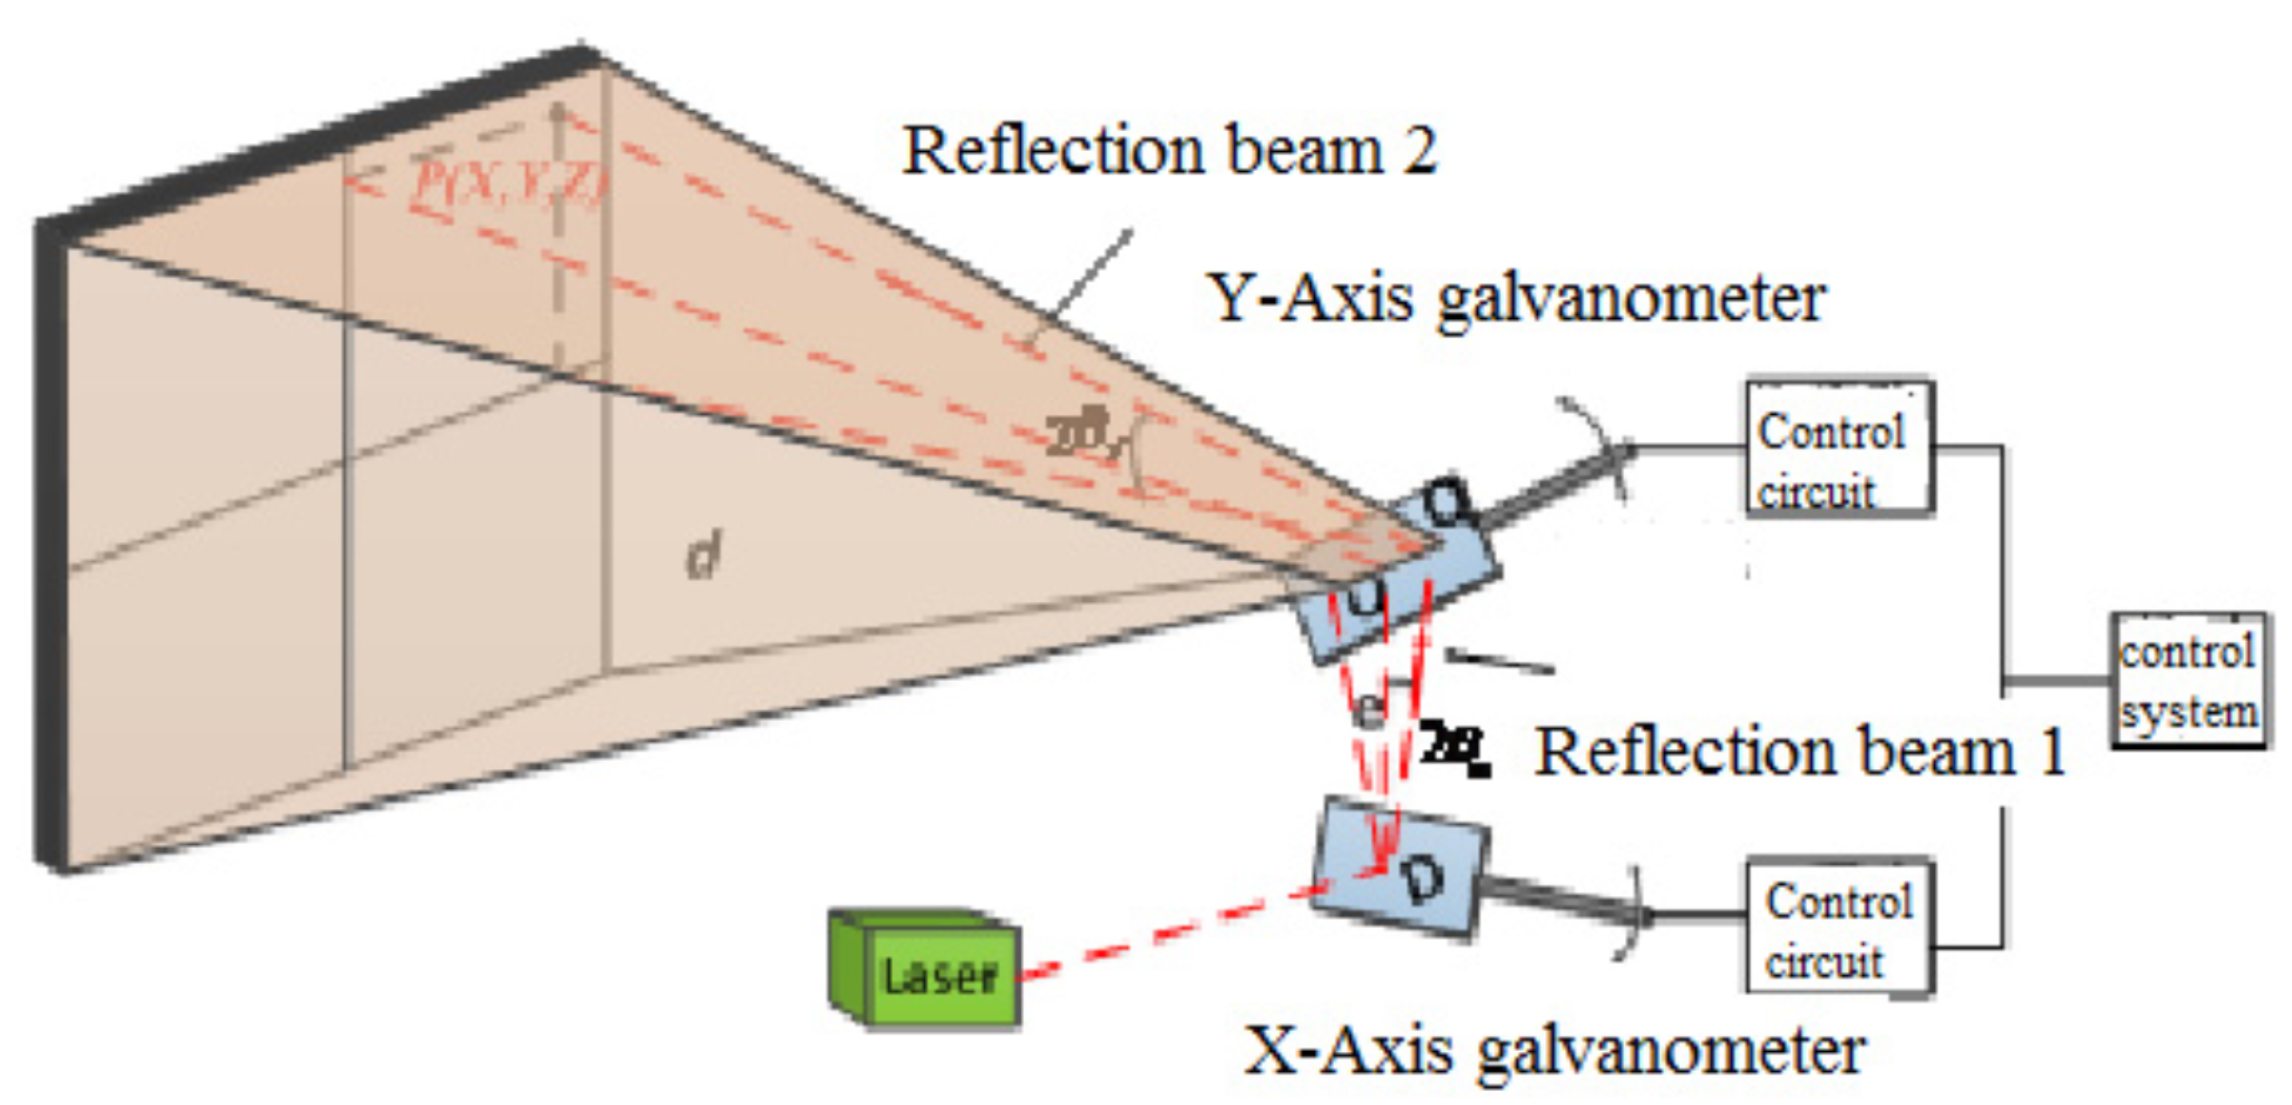
\includegraphics[width=15cm]{img/optics.png}
\caption{Model of the optical mirror system \cite{Meng.2019}}
\label{optics}
\end{center}
\end{figure}
Because the scanner can only indirectly control the laser dot on the working plane by turning its mirrors, some sort of mathematical representation of this system must be derived. This representation will used for turning XY-directions into mirror rotation angles. From \cite{Meng.2019} we get the following equations:
\begin{equation}\label{eqn1}
x=e\cdot tan(2\theta_x)+tan(2\theta_x) \cdot \sqrt{d^2+y^2} 
\end{equation} 
\begin{equation}\label{eqn2}
y = d\cdot tan(\theta_y)
\end{equation} 
where $x$ and $y$ are the point coordinates on the plane, $\theta_x$ and $\theta_y$ are the rotations angles of the mirrors\footnote{More specifically: $\theta_x$ is the angle between the laser beam and the first reflection beam minus $90^\circ$. Similarly, $\theta_y$ is the angle between the first and second reflection beam minus $90^\circ$.}, $e$ is the vertical distance between the mirror axes and $d$ is the normal distance between the projection plane and the Y-mirror rotation axis. \\
Since $x$ and $y$ are given by the user (rather the gcode), equations \ref{eqn1} and \ref{eqn2} must be solved for $\theta_x$ and $\theta_y$. These angles will be turned into step signals for the steppers. From equation \ref{eqn2} we can derive 
\begin{equation}\label{eqn3}
\theta_y = \frac{arctan(\frac{y}{d})}{2}
\end{equation} 
From equation \ref{eqn1}, $\theta_x$ can be found:
\begin{equation}\label{eqn4}
\theta_x=\frac{arctan\left( \frac{x}{e+\sqrt{d^2+y^2}}\right) }{2}
\end{equation}
Looking at figure \ref{optics}, $x$ and $y$ must be zero, when $\theta_x=\theta_y=0^\circ$ \footnote{with these angles, all beams are orthogonal. This configuration is referred to the neutral or home position.}. Equations \ref{eqn3} and \ref{eqn4} confirm this. 

\section{Implementation}
In this section, construction details of the galvo scanner will be explained.
\subsection{Mechanics and Optics}
\begin{figure}[H]
\begin{center}
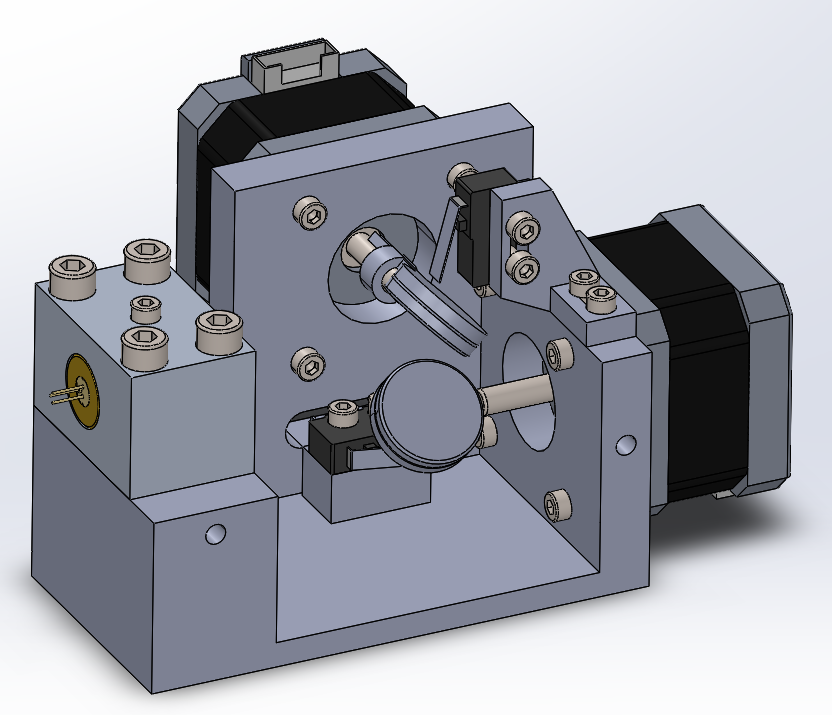
\includegraphics[width=15cm]{img/mechanics.png}
\caption{CAD-Rendering of the mechanical system}
\label{mechanics}
\end{center}
\end{figure}
The mechanics of this design are relatively simple: The mirrors are attached to stepper motors by glueing aluminium holders onto the flat piece of the rotor and glueing the mirrors (in this case 20x3mm molybdenum mirrors) onto the holder and the rotor\footnote{The holders were machined and 3D-printed (PLA, 100\% infill) to test the difference in performance, but none was noticeable. The molybdenum mirrors are relatively heavy, but are the cheapest viable option available.}. The motors are then screwed onto the 3D-printed base (PLA, 60\% infill). This base also has features to screw on endswitches (for homing the mirrors) and the laserdiode array. The latter consists of a machined aluminium block into which the laserdiode holder (machined brass) fits. This holder also has a M9x0.5 thread for the collimator unit. The collimator can be adjusted via this thread. \\
\subsection{Electronics}
\begin{figure}[H]
\begin{center}
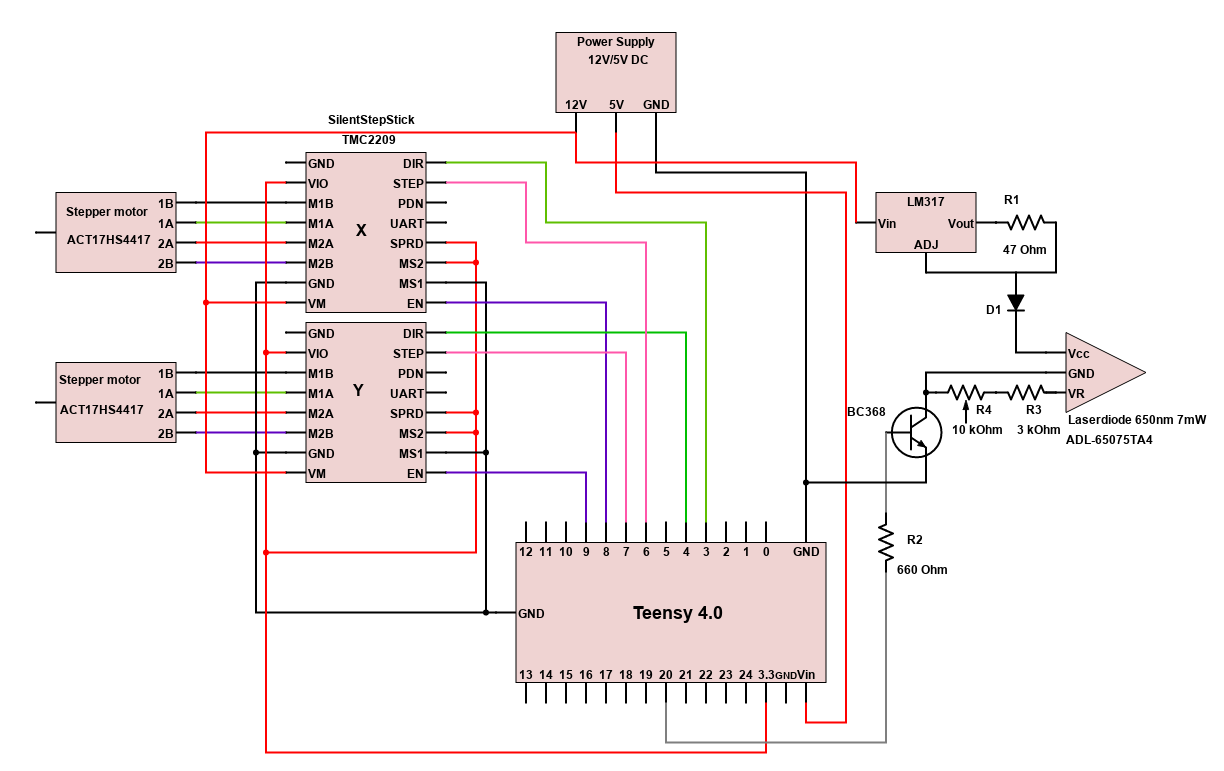
\includegraphics[width=15cm]{img/electronics.png}
\caption{Wiring diagram for the system}
\label{electronics}
\end{center}
\end{figure}
Figure \ref{electronics} shows the electrical diagram of the system. The stepper motors are Nema-17 ACT 17hs4417 steppers. The SilentStepSticks (containing Trinamic TMC2209 ICs)  were chosen as drivers because of their high micro-stepping capabilities (up to 256), extremely low noise and relatively low cost (about 10 Euros or 12 USD per driver). \\
For the main controller, a Teensy 4.0 was chosen because of the extremely high clock frequency of 600Mhz\footnote{In comparison, an Arduino Nano only has 16MHz clock frequency!} and its easy programmability through the Arduino IDE. It must be noted, that the Teensy 4.0 only tolerates 3.3V logic voltage. 

\paragraph{Note:} Teensy Boards and laserdiodes can be very fragile electrical components (multiple Teensies and Diodes were destroyed in this project), so it may be worth the money and effort to use an Arduino in order to test the circuits/code and use dummy loads for simulating laser diodes. Since the SilentStepStick-Drivers can tolerate 3.3V and 5V as logic voltages, the microcontrollers can be changed without changing the circuit. However, the footprints are not equal, so jumper cables are necessary for replacing the Teensy with an Arduino. \\

For driving the laserdiode, a special diode driver is used, which can supply 0-500mA of constant regulated current\footnote{It is possible to use a LM317 and correct resistors for a constant current source. This was tested in this project, but resulted in a lot of destroyed laser diodes, which is why a complete driver circuit was bought.}. \\
This driver circuit is activated by a NPN-Transistor (specifially, a BC368). For calculating its base resistance $R_2$, a base current of the BC368 transistor of $I_B=5mA$ is selected \cite[p. 3]{SemiconductorComponentsIndustries.2007}. Since the Teensy 4.0 logic voltage is $3.3V$, a resistance value of $R_2=\frac{3.3V}{5mA}=660\Omega$ is selected. \\
The laser diode has three pins: \textit{Vcc}, \textit{GND} and \textit{VR}. \textit{Vcc} is connected to the output of the constant current source, \textit{GND} is connected to the \textit{Laser -} pin of the diode driver. \textit{VR} is connected to \textit{Laser -} via a resistance of $3k\Omega$ (maximum power) - $13k\Omega$ (minimum power), which is realised with fixed resistors ($3.2k\Omega$) in series with a linear potentiometer ($10k\Omega$). The GND of the diode driver is connected to a transistor to switch it on or off.\\
For supplying Vcc (5V) for the Teensy and the laser driver, a LM317 linear voltage regulator is used in the shown configuration. The resistors $R_1$ and $R_2$ can be computed as follows \cite[p. 10]{lm317}: 
\begin{equation}
V_{out} = 1.25 \cdot \left( 1+\frac{R_2}{R_1} \right)
\end{equation}
$V_{out}$ must be 5V and $R_1$ is chosen to be $1k\Omega$. Therefore, $R_2$ must be:
\begin{equation}
R_2 = \left( \frac{V_{out}}{1.25V} - 1 \right) \cdot R_1 =  \left( \frac{5V}{1.25V} - 1 \right) \cdot 1000\Omega = 3000\Omega
\end{equation}
$R_4$ and $R_5$ are pull-down resistors that draw the pin state of pins $9$ and $10$ (pins for the endstops) to the low state to prevent undefined behaviour. \\
$JP_1$ and $JP_2$ are jumpers that set the microstepping mode of the stepper motor drivers to $\frac{1}{8}$ (jumper disconnected) or $\frac{1}{64}$ (jumper connected).
\subsection{Code}
\begin{figure}[H]
\begin{center}
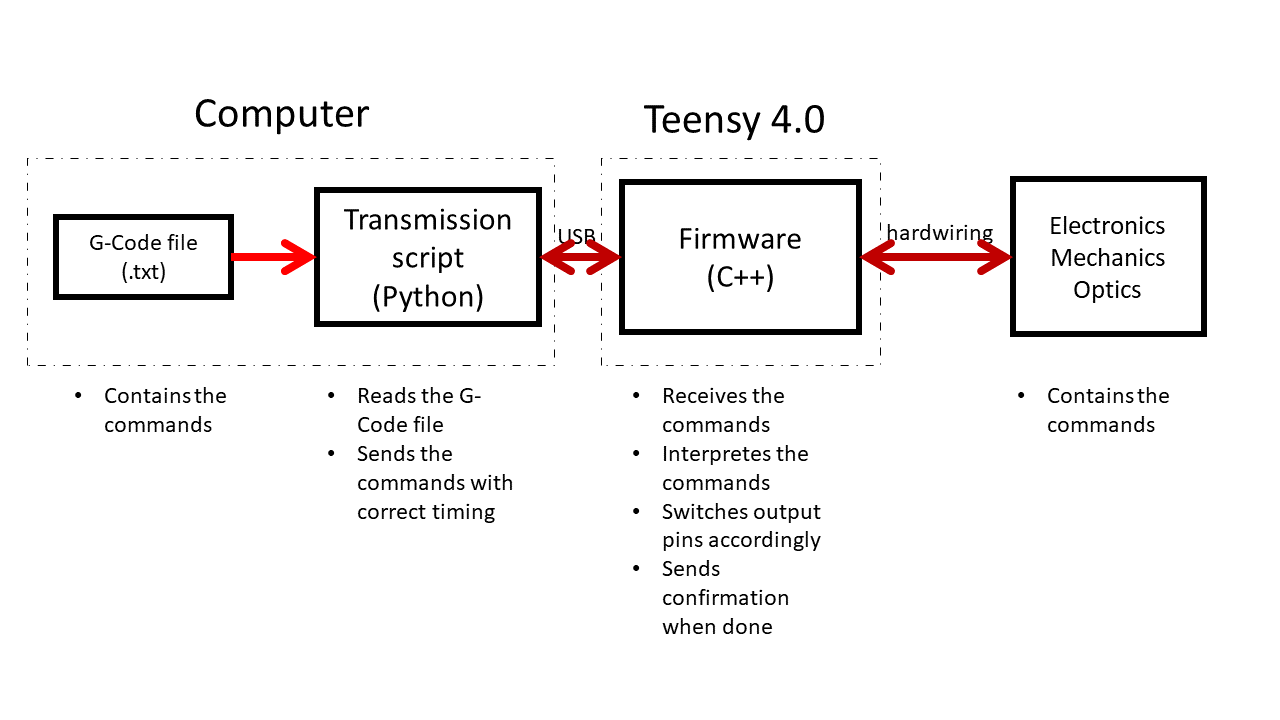
\includegraphics[width=15cm]{img/programArchitecture.png}
\caption{A simplified diagram of the program architecture}
\label{code}
\end{center}
\end{figure}
The programm architecture (see figure \ref{code}) consists of three main parts: The teensy firmware, a python script for Gcode transmission and the G-Code itself. 
\paragraph{Firmware}
The firmware is the most critical part of the architecture: It interpretes the received (via Serial) G-Code commands and coordinates all of the outputs and inputs, such as step and direction signals and the transistor base for the laser or the endstop signals. Because it is directly compiled onto the Teensy via the Arduino IDE, it is written in C++.\\
The firmware supports the following G-Code commands: G0, G1, G2, G3, G28, G60, G61, M3, M4, M5, M201, M203. \footnote{For a detailled explanation and syntax details, see the GalvoStep wiki at \url{https://github.com/NiklasHammerstone/GalvoStep}} The firmware sends a short confirmation (usually: \textit{OK}), when the command is processed. If it included stepper movement (such as G0), the confirmation will only be sent when steppers have reached their target position.
\paragraph{Transmission script}
The transmission script is a Python script that reads the G-Code file from a specified location on the PC. The gcode is read, encoded and sent via a Serial connection (USB). Before the next line is sent, the script waits for a confirmation from the firmware. This makes sure that no command is sent before the firmware is finished processing the previous command. This loop is repeated until no G-Code commands are left to send.
\paragraph{G-Code}
The G-Code file is a simple text file (.txt) which contains the command lines. It is critical that each line only contains one command. \\


\section{Results}
\subsection{General functionality}
The proposed functionality was realised. The prototype can be given commands by sending G-Code commands via the Arduino IDE Serial Monitor or a Python script\footnote{The code files can be downloaded via GitHub: \url{https://github.com/NiklasHammerstone/GalvoStep}}. The commands are executed instantly. No delay between commands is perceivable when a whole G-Code file is executed via the Python script. This results in a smooth movement of the laser spot. \\
A G-Code file drawing a heart shape was tested with step frequencies of $2000 \frac{steps}{s}$ up to $20000\frac{steps}{s}$ and a distance from the projection plane of about $200mm$. At about $10000-12000 \frac{steps}{s}$ the moving spot started to look like a (more or less) stationary image\footnote{This is only true for the naked eye. Also, the border step frequency is dependent on the size of the image, the background, the laser intensity and the general lighting of the room.}, with the shape of the image still not being noticeably distorted. At about $15000-18000 \frac{steps}{s}$ the image stationarity was satisfactory, but mechanical vibrations led to a distorted image. The results of this test can be seen in figures \ref{slow} and \ref{fast}. 
\begin{figure}[!h]
\noindent
\begin{minipage}{0.4\textwidth}%
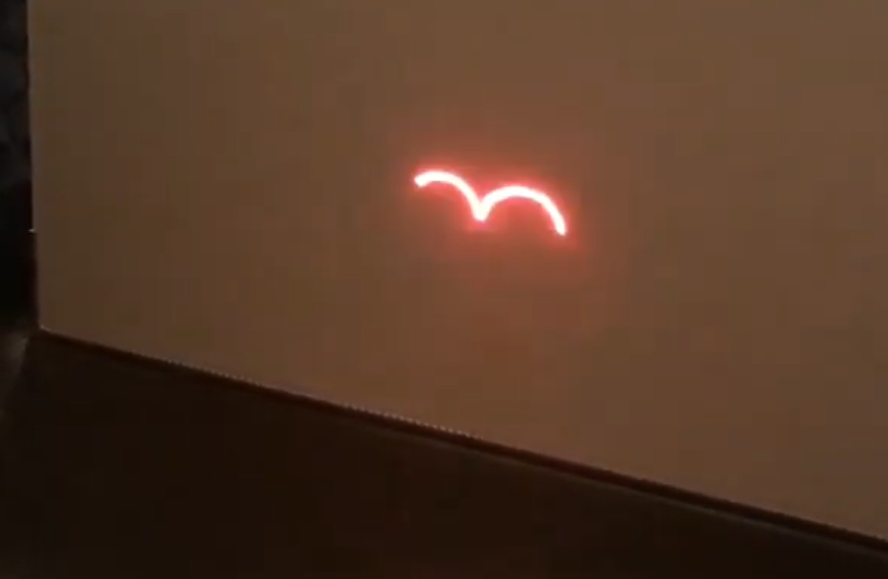
\includegraphics[width=\textwidth]{img/hearttestslow}
\caption{Arcs of the projected heart at $8000 \frac{steps}{s}$}
\label{slow}
\end{minipage}%
\hfill
\begin{minipage}{0.4\textwidth}%
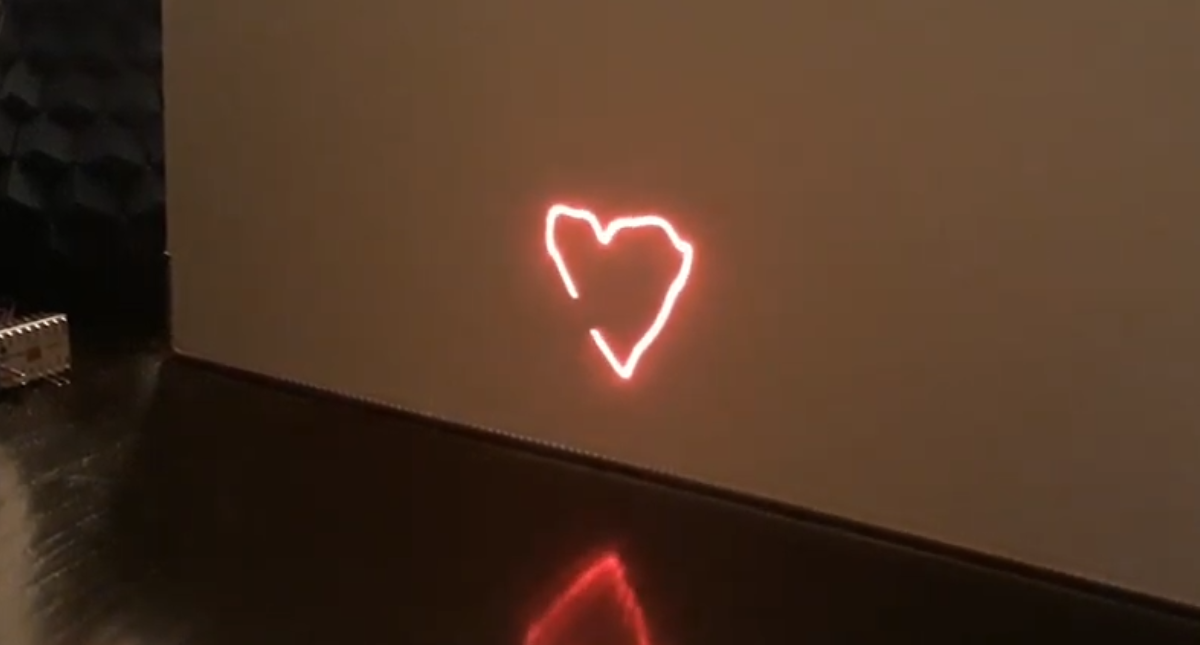
\includegraphics[width=\textwidth]{img/hearttest}
\caption{Almost entire heart at $20000 \frac{steps}{s}$}
\label{fast}
\end{minipage}%
\end{figure}
Note that the rolling shutter of the camera is quite fast, which is why only the picture at about $20000 \frac{steps}{s}$ is (almost) completely visible in one photo. However the difference of the arcs alone should convey the diffence of the whole picture. \\
\subsection{Accuracy and precision}
\begin{figure}[H]
\begin{center}
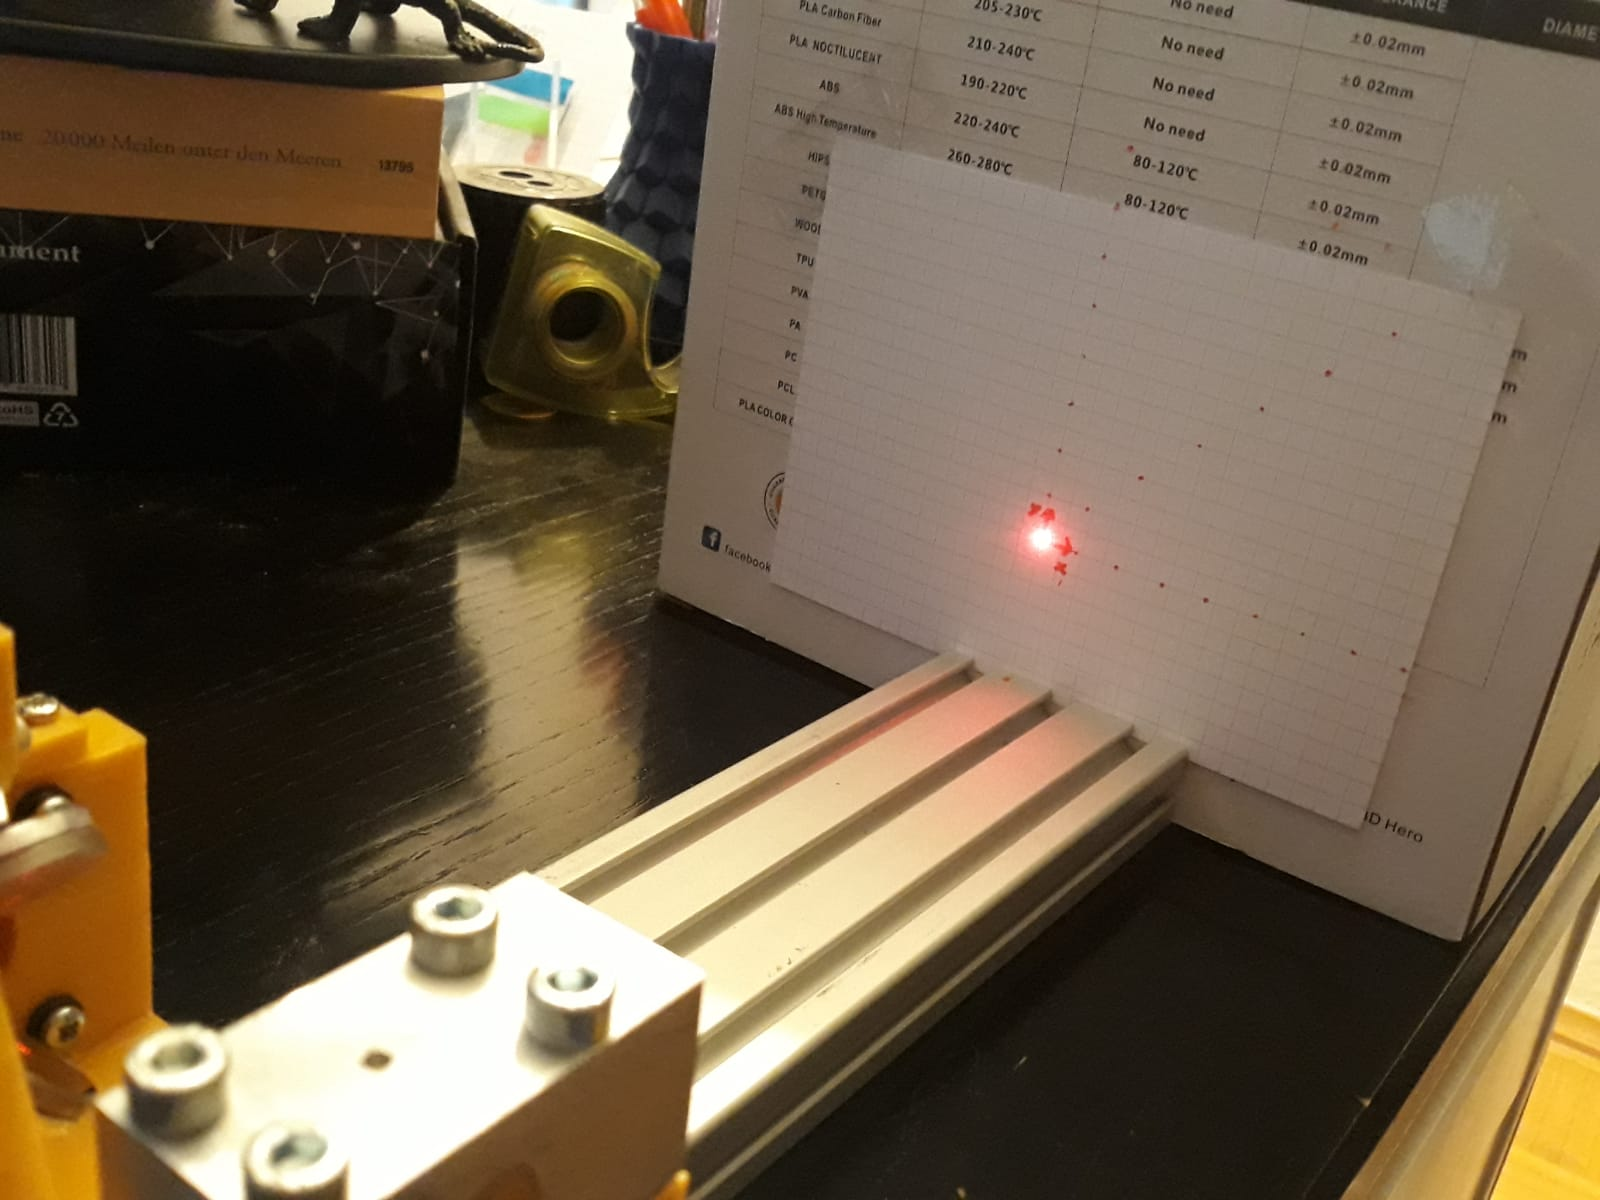
\includegraphics[width=15cm]{img/testprocedure.jpeg}
\caption{Snapshot of the testing procedure}
\label{testing}
\end{center}
\end{figure}
In order to test the accuracy of the prototype, the following procedure was performed:
\begin{enumerate}
\item Place the machine in front of a plane with a defined distance D.
\item Home the mirrors.
\item Move the laser point in 10mm steps in X-, Y-, and XY direction (from -20 to +80) with speed F.\footnote{An example command for testing the XY direction would be \textit{G0 X20 Y20}. In this test, X and Y coordinates were always equal to reach an ideal line of slope 1.}
\item Mark the actual laser spot carefully with a pen for each step (see figure \ref{testing})\footnote{Since the prototype utilizes a 7mW laser diode, the laser itself is too weak to mark the paper by itself.}
\item After the testing is done, measure the actual distances of the spots from the origin point.
\end{enumerate}
From the Y-, X- and XY, the average and maximum difference from the ideal coordinates are computed. For the XY-coordinates, average slope and intercept were calculated to analyze the linearity of the system.
\begin{figure}[H]
\begin{center}
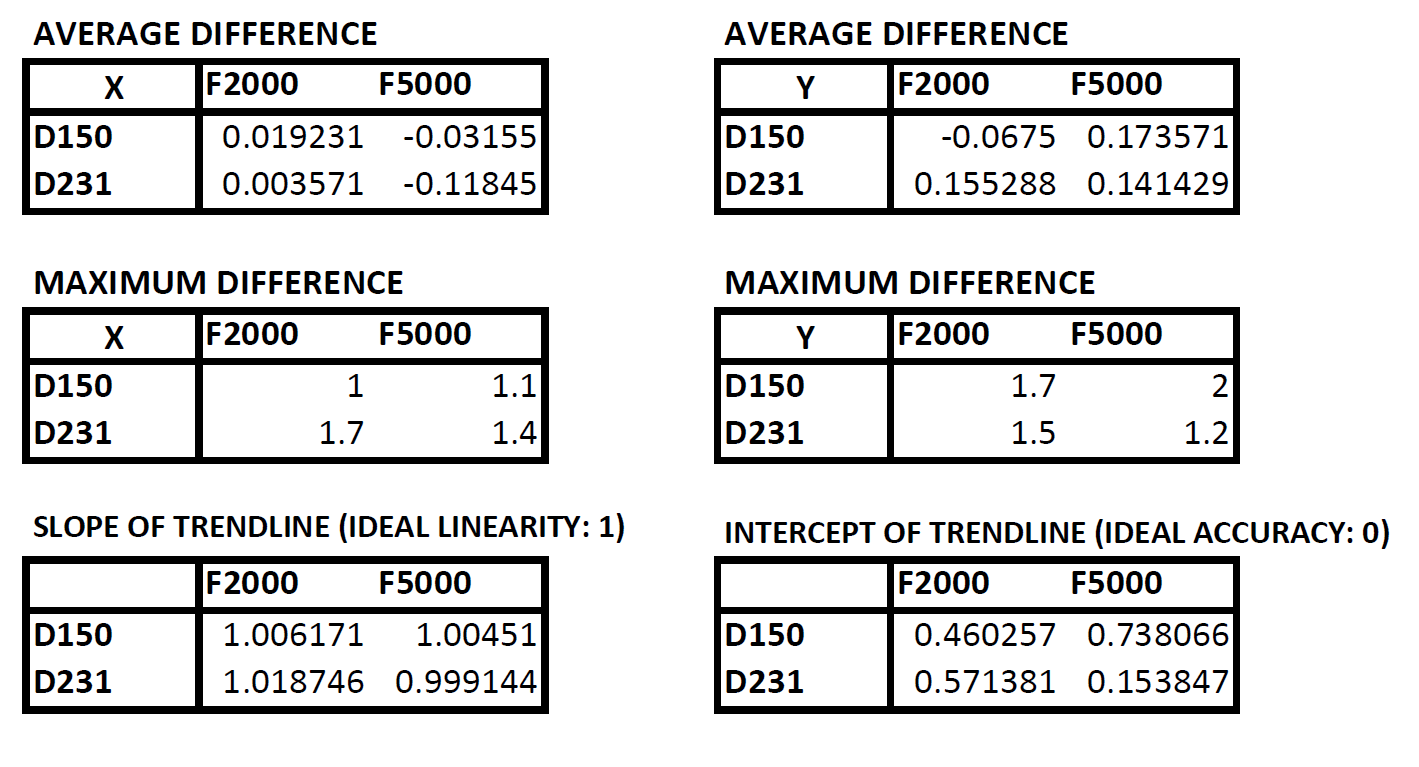
\includegraphics[width=15cm]{img/accuracy.png}
\caption{Results of the accuracy analysis}
\label{results}
\end{center}
\end{figure}
In figure \ref{results} the results of the mentioned tests are shown. It is expected, that the average and maximum differences (representing positional accuracy) would rise with rising distance \textit{D} and feedrate \textit{F}. However, no such trends can be seen from the data. The average difference is consistently lower than $0.2mm$, but the absolute maximum is $2mm$. This suggests relatively high accuracy, but low precision. This is verified by the slope of the trendline for the XY-point testing. The highest difference from the ideal slope of 1 (since the same values were used for X and Y coordinates simultaneously) was $0.018\frac{mm}{mm}$, suggesting high accuracy. However, the intercepts of the trendlines (ideal would be zero) differ widely from zero, with differences going as high as $0.738mm$, suggesting low precision. This result suggests that the machine is working correctly\footnote{\glqq Working correctly\grqq refers to the mathematic model being correct and the physical, electrical and optical design being expedient in theory}, but is lacking the mechanical alignment for high precision.\\ 
Furthermore, the repeatability of the endstops and backlash of the motors was tested. For the repeatability test of the endstops, the machine was homed ten times (homing speed: $500\frac{steps}{s}$) and the spot offsets were noted. The average difference was about $0.3mm$ with a maximum of $2mm$, resulting in a arc accuracy of $0.5^\circ$. These inaccuracies are most likely due to the cheap mechanical endstops used.\\
For the backlash test, the machined was homed and the spot was moved by $80mm$ back and forth multiple times in X and Y directions. As expected (because no parts are present that could induce backlash), no backlash was perceivable.
\subsection{Flaws of the testing methodology} It must be noted that the proposed method of testing has inherent inaccuracies: Since the laser can not mark paper by itself, it is necessary to use a pen, but as soon as the pen is brought into position, it blocks the laser beam. This way its necessary for the operator to visually remember where the spot was. The marked spot can be checked by removing the pen and therefore unblocking the pen, but since both the spot and the pen marking have a diameter of approximately $1.5mm$\footnote{The actual laser spot is much smaller than this, but appears to be larger due the light  being scattered and dispersed in the surrounding paper}, this method can not guarantee results within about half of that range ($0.5 - 0.9 mm$). This can be partly compensated by making sure that the caliper blades are positioned in the exact middle (which itself is only possible within a few tenths of a millimeter) of the pen marking when measuring the points. Also, the paper pieces used for this test did bow out by approximately $1mm$, which is unideal. In conclusion, the difference of laser spot and pen marking and the measuring inaccuracies add up to such a big margin of error (approximately $\pm 1mm$) that the exact values of the point coordinates are relatively useless for accuracy analysis. However, since the presented flaws are unsystematic and randomn (except for the bow of the paper), the averages (average distance, slope and intercept of trendline) should be more conclusive. \\
These flaws can be elimininated entirely by using a more powerful laser which can mark wood by itself. This would eliminate the pen method with all its flaws and inaccuracies and only leave the direct measuring inaccuracies of the calipers, which are usually within $0.02 - 0.1mm$. \\

\section{Conclusion}
In conclusion, the goal of a proof-of-concept for a steppermotor-actuated galvoprojector was reached. The machine can be used via G-Code like a normal CNC-machine (e.g. 3D-printer, CNC-Router) and can draw figures with step speeds of up to $20000 \frac{steps}{s}$, depending on how much distortion is acceptable for the user. Since this machine cannot compete with laser projectors using real galvoactuators, its most probable usecase would be engraving with speeds unreachable for most CO2 or diode daser machines currently on the market. Since the precision of the current prototype is quite limited (as shown in the chaper Results), more work is required to be able compete with normal benchtop laser engravers (see Prospect).
\section{Prospect}
In the following versions of this machine, the steppermotors and endstops will be upgraded. The base will be re-designed to fit the new high-power laser module and the mirrors will be replaced. An F-theta objective might be added to increase light intensity at the working plane and therefore engraving speed. Finally, safety precautions (Enclosure with laser windows and doorswitch) will be added to shield the laser beam. The electronics will not be changed much, since they worked without problems\footnote{Maybe a PCB will be designed and manufactured for the schematic.}. 
\section{Acknowledgements}
Special thanks to the members of the forum \url{www.laser-engravers.de}, especially \glqq VDX \grqq and \glqq Gewindestange\grqq, without which a lot more laser diodes would have been destroyed in the process of this project.

\addcontentsline{toc}{section}{References}
\bibliography{literature}
\end{document}